% -*- mode: LaTeX; coding: utf-8 -*-
% Typeset with: XeLaTeX

\documentclass{beamer}
\mode<presentation>
{
  \usetheme[progressbar=foot,numbering=fraction,background=light]{metropolis} 
  \usecolortheme{default} % or try albatross, beaver, crane, ...
  \usefonttheme{default}  % or try serif, structurebold, ...
  \setbeamertemplate{navigation symbols}{}
  \setbeamertemplate{caption}[numbered]
  %\setbeamertemplate{frame footer}{My custom footer}
}
\centering

\usepackage{graphicx}
\graphicspath{ {./fr_figures/} }
\usepackage{hyperref,xcolor}
\newcommand{\link}[2]{\href{#1}{\textcolor{blue}{\underline{#2}}}}

% Main document
\begin{document}
\title{DeepSite: NNets for binding site prediction}
\subtitle{Algorithms in Structural Bioinformatics}
\author{Thomas Pappas}
%\date{4 March 2020}
\maketitle

\begin{frame}{Agenda}
  \tableofcontents[hideallsubsections]
\end{frame}

\section{What is the project about?}

\begin{frame}{What is DeepSite?}
  \begin{block}{DeepSite}
    Protein-binding site \emph{predictor} using 3D-convolutional neural networks
  \end{block}
  \begin{block}{}
    DeepSite is an algorithm that given a protein it returns predictions about its binding pockets.
    It uses a Deep Convolutional Neural Network (DCNN) which is trained from an existing database of 7622 protein-binding sites (scPDB).
      %\item Superior performance to two other competitive algorithmic strategies
  \end{block}
  \begin{block}{}
      DeepSite is available online at \link{https://www.playmolecule.com/deepsite/}{https://www.playmolecule.com/deepsite/}
  \end{block}
\end{frame}

\begin{frame}{Aim and objectives of the project}
  \begin{block}{}
    In this project we will be focusing on the following:
  \end{block}
  \begin{block}{Review}
    First we will analyse how the algorithm works, i.e. how it converts a protein structure into an input for the DCNN, how is the later structured and how it uses its results to make predictions about the protein's binding sites?
  \end{block}
  \begin{block}{Confirm}
    % TODO: Add the new number of scPDB available data to date.
    The algorithm's DCNN was trained using the scPDB data available in 2017. Since then scPDB has gathered more data which gives us a great dataset to test and verify the accuracy of the algorithm.
  \end{block}
  \begin{block}{Compare}
    Investigate the algorithm's results and performance compared to other binding site prediction ones, and more specifically with the fpocket algorithm.
  \end{block}
\end{frame}

\begin{frame}{Challenges}
  \begin{block}{}
    Most of the challenges for this project derive from the fact that the algorithm was not reconstructed.
    While parts of the algorithm are included in the paper, due to lack or time, resources and expertise of the author, re-implementation was not possible.

    For this reason the \link{https://www.playmolecule.com/deepsite/}{DeepSite web app} was used to get the algorithm's output for a given protein.
  \end{block}
  \begin{block}{}
    Therefore
    \begin{itemize}
      \item The DCNN training and performance couldn't be evaluated
      \item In the review and comparison sections, the volumentric map of the binding site could not be utilised and thus focus has been put on the center $3D$ coordinates of the pocket
    \end{itemize}
  \end{block}
\end{frame}

\begin{frame}{Challenges}
  \begin{block}{}
    Another challenge in reviewing comes from the fact that the sc-PDB database provides very few binding site pocket for a given protein. Since the DeepSite algorithm can return multiple pocket predictions, we can only validate those available using the scPDB data.
  \end{block}
\end{frame}

\section{The DeepSite algorithm}

\begin{frame}{The DeepSite Algorithm}
  \begin{block}{I/O Overview}
    \begin{itemize}
      \item Input: A protein ID or a PDB file
      \item Output: A list of pocket predictions
      \begin{enumerate}
        \item Volumetric map of the protein's probability to have a pocket in a specific voxel, clustered in the different predictions
        \item 3D coordinates of the voxel with the highest probability in each cluster
        \item Prediction score
      \end{enumerate}
    \end{itemize}
  \end{block}
  \begin{block}{I/O Example}
    \begin{itemize}
      \item Input: "6FAT" (protein ID)
      \item Output (Volumetric map not utilised):
      \begin{enumerate}
        \item $\left[-1.4, 61.0, 69.6\right], 1.0$
        \item $\left[4.6, 37.0, 49.6\right], 0.94$
      \end{enumerate}
    \end{itemize}
  \end{block}
\end{frame}

\begin{frame}{Example of a 6FAT protein}
  \begin{figure}[h]
    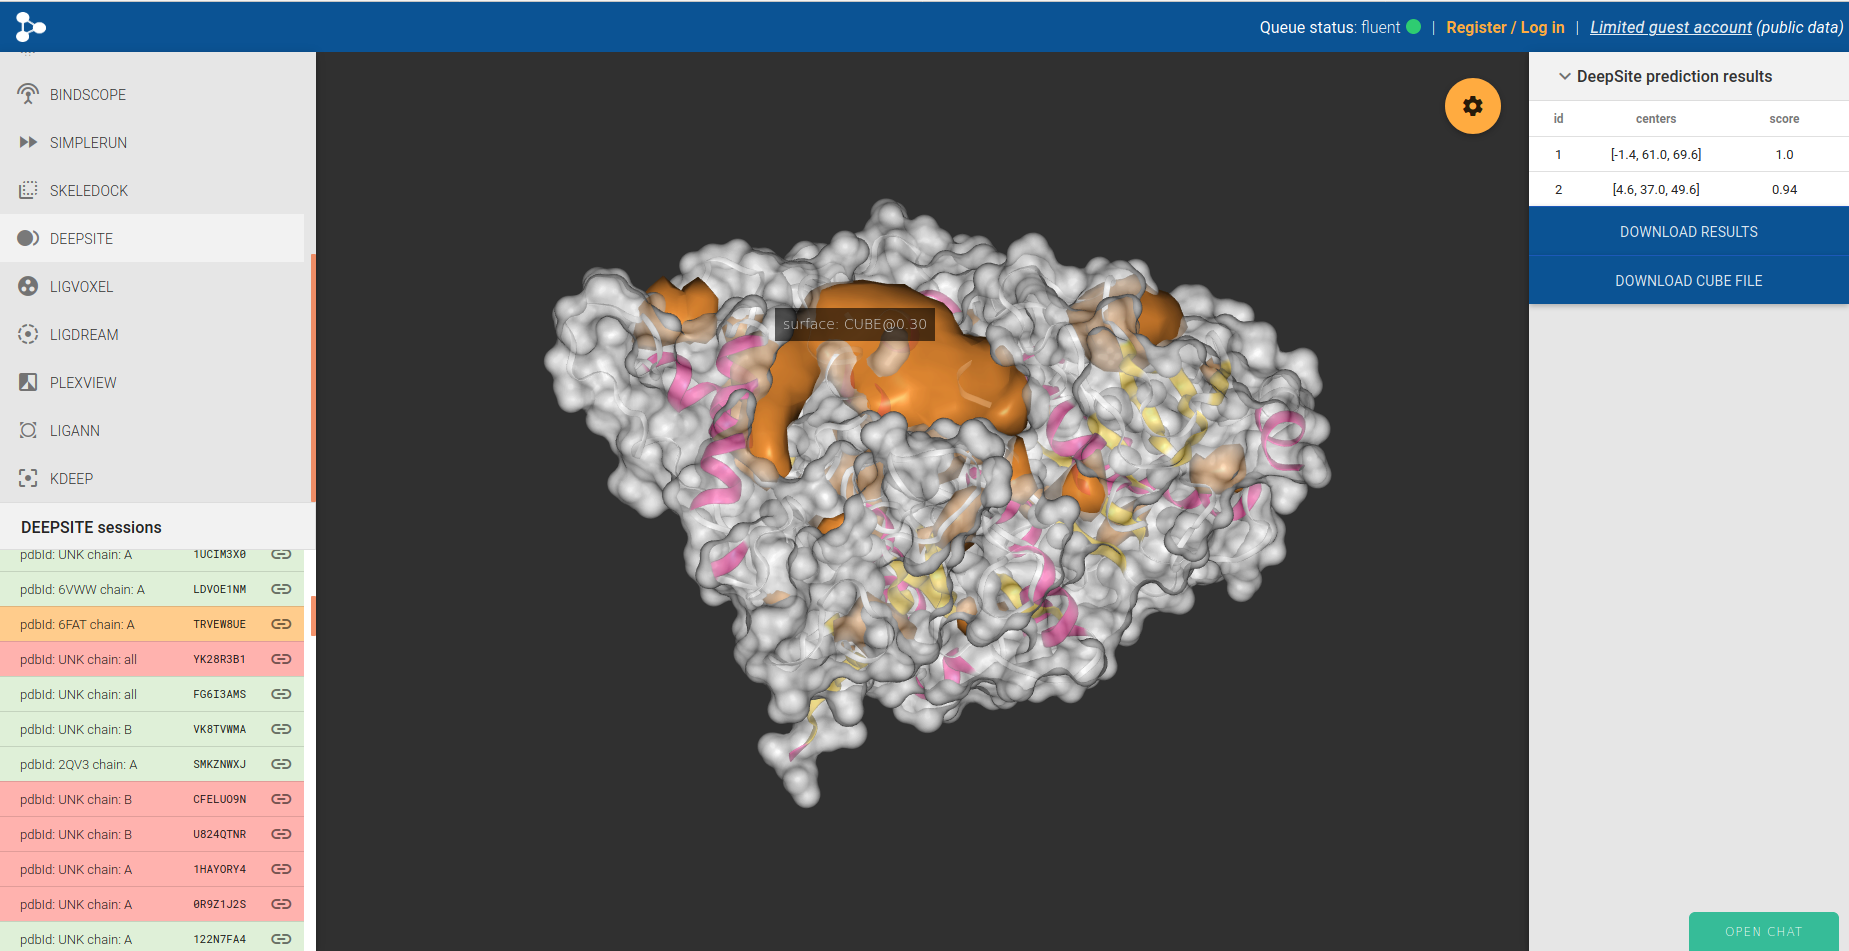
\includegraphics[width=1\textwidth]{deepsite_6fat_result}
    \caption{The 6FAT protein submitted in the \link{https://www.playmolecule.com/deepsite/}{DeepSite web app}}
  \end{figure}
\end{frame}

\begin{frame}{The DeepSite Algorithm}
  \begin{block}{Algorithm steps (summary)}
    \begin{enumerate}
      \item Take as input a protein ID or a PDB file and parse the DB atom coordinates to a grid
      \item Create 8 more grids, one for each protein property
      \begin{itemize}
        \item Each property grid is a probability map i.e. each voxel contains the probability of an atom of that property to be within it
        \item Each property grid is a Neural Network (NNet) channel
      \end{itemize}
      \item Take all $16 \times 16 \times 16$ \AA$^3$ subgrids from the 8 channels and give it as input to the DCNN
      \begin{itemize}
        \item The DCNN will return the probability for the center of the input subgrid to be in a binding site pocket
        \item Creates a probability map for all voxels of the protein
      \end{itemize}
    \end{enumerate}
  \end{block}
\end{frame}

\begin{frame}{The DeepSite Algorithm}
  \begin{block}{Algorithm steps (summary)}
    \begin{enumerate}
      \setcounter{enumi}{3}
      \item Use the Mean Shift (Comaniciu and Meer, 2002) clustering algorithm to distinquish the different binding site pockets
      \item Take the voxel with the max probability from each cluster and return its coordinates and its score
    \end{enumerate}
  \end{block}
\end{frame}

\subsection{Steps 1 & 2: Translating PDB to NNet channels}

\begin{frame}{Translating PDB to NNet channels}
  \begin{block}{Step 1: Parse the PDB data}
    \begin{itemize}
      \item Parse the atom coordinates from the PDB data
      \begin{itemize}
        \item Use of the HTMDs (Doerr et al., 2016) Python package
      \end{itemize}
      \item Consider the space grid containing the protein
      \begin{itemize}
        \item Grid is split to $1 \times 1 \times 1 $ \AA$^3$ voxels
        \item $+8$\AA \;for the cases where the binding pockets are on the edge
      \end{itemize}
    \end{itemize}
  \end{block}
%\end{frame}

%\begin{frame}{Translating PDB to NN channels}
  \begin{block}{Step 2: Generate the 8 protein-property grids/channels}
  Using the AutoDock 4 tables (Tables \ref{table:1} \& \ref{table:2}), for each of the 8 protein properties we do the following:
    \begin{itemize}
      \item Filter the atoms that have that property
      \item Create a grid and for each voxel calculate the atom occupancy, i.e. the probability for the voxel to contain an atom of that property
    \end{itemize}
  \end{block}
\end{frame}

\begin{frame}{AutoDock 4 tables}
  \begin{columns}
    \begin{column}{.4\textwidth}
      \begin{tiny}
      \begin{table}
      \caption{Atom types}
      \label{table:1}
      \begin{tabular}{ l l }
        \hline
        Element & Description \\
        \hline
        C & Non H-bonding aliphatic carbon \\
        A & Non H-bonding aromatic carbon \\
        NA & Acceptor 1 H-bond nitrogen \\
        NS & Acceptor S Spherical nitrogen \\
        OA & Acceptor 2 H-bonds oxygen \\
        OS & Acceptor S Spherical oxygen \\
        SA & Acceptor 2 H-bonds sulfur \\
        HD & Donor 1 H-bond hydrogen \\
        HS & Donor S Spherical hydrogen \\
        MG & Non H-bonding magnesium \\
        ZN & Non H-bonding zinc \\
        MN & Non H-bonding manganese \\
        CA & Non H-bonding calcium \\
        FE & Non H-bonding iron \\
        \hline
      \end{tabular}
      \end{table}
      \end{tiny}
    \end{column}
    \begin{column}{.6\textwidth}
      \begin{tiny}
      \begin{table}
      \caption{Property-atom type correspondence}
      \label{table:2}
      \begin{tabular}{ l l }
        \hline
        Property & Rule \\
        \hline
        Hydrophobic & atom type C or A \\
        Aromatic & atom type A \\
        Hydrogen bond acceptor & atom type NA or NS or OA or OS or SA \\
        Hydrogen bond donor & atom type HD or HS with O or N partner \\
        Positive ionizable & atom with positive charge \\
        Negative ionizable & atom with negative charge \\
        Metal & atom type MG or ZN or MN or CA or FE \\
        Excluded volume & all atom types \\
      \end{tabular}
      \end{table}
      \end{tiny}
    \end{column}
  \end{columns}
  Table 1, Table 2, 10.1093/bioinformatics/btx350
\end{frame}

\begin{frame}{Translating PDB to NNet channels}
  \begin{block}{Atom occupancy}
    We calculate the probability of an atom of distance $r$ to the center of a voxel by using the pair correlation function.
    \[
      g(r) = exp(-\beta V(r))
    \]
    where $V(r) = \epsilon (r_{vdw}/r)^{12}$ and by taking $\epsilon = \beta^{-1}$ we get the \emph{single atom occupancy estimate} to be
    \[
      n(r) = 1 - exp(-(r_{vdw}/r)^{12})
    \]
  \end{block}
  \begin{block}{Building the NNet channels}
    For each channel we through each voxel and for each we calculate $n(r)$ for all atoms in the protein and assign to it the max value. This way we end up with 8 3D matrices where each voxel has the probability of having an atom of that property in them (Figure 2)
  \end{block}
\end{frame}

\begin{frame}{Translating PDB to NNet channels}
  \begin{figure}[h]
    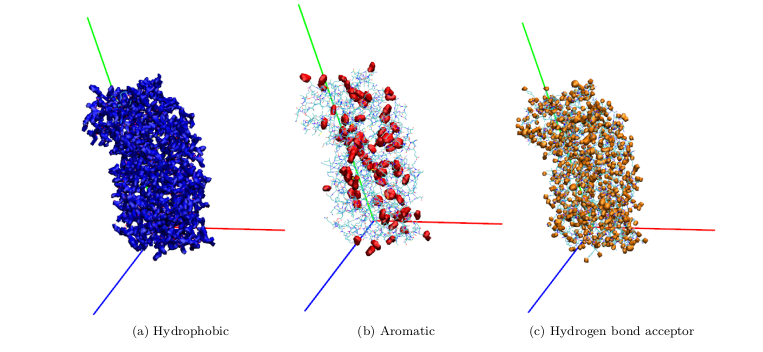
\includegraphics[width=1\textwidth]{deepsite_protein_property_channels}
    \caption{Visual representations of descriptor channels (3/8) for PDB ID 4NIE, Figure S2, 10.1093/bioinformatics/btx350}
  \end{figure}
\end{frame}

\subsection{DCNN design}

\begin{frame}{DCNN design}
  \begin{block}{}
    Before we move on to Step 3., let's take a look at the DCNN design and architecture.

    The DCNN takes as input $8$ 3D matrices of size $16 \times 16 \times 16$ and outputs a value between $0$ and $1$ (probability).

    In context (after it is trained), it takes subgrids of the 8 protein property channels and then calculates the probability of the center voxel of that subgrid to be a binding site pocket.
  \end{block}
\end{frame}

\begin{frame}{DCNN design}
  \begin{figure}[h]
    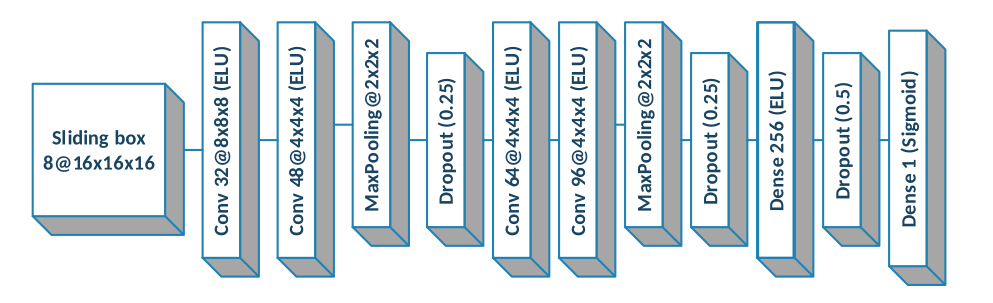
\includegraphics[width=1\textwidth]{deepsite_dcnn_architecture}
    \caption{DeepSite’s internal DCNN architecture, Fig. 2, 10.1093/bioinformatics/btx350}
  \end{figure}
\end{frame}

\begin{frame}{DCNN properties}
  \begin{block}{Layers}
    \begin{itemize}
      \item 4 Convolutional Layers
      \item Max Pooling and Dropout layers after each 2
      \item Sigmoid activation function at the end to get a probability
    \end{itemize}
  \end{block}
  \begin{block}{But why such a structure was chosen?}
    \begin{itemize}
      \item Common practices in the ML community
      \item Simplified model due to scarcity of data
      \item Variations have been attempted with no apparent differences
    \end{itemize}
  \end{block}
\end{frame}

\begin{frame}{DCNN properties}
  \begin{block}{Issues}
    \begin{itemize}
      \item Class imbalance problem since most protein subgrids are not close to a binding site
      \begin{itemize}
        \item Tackled by undersampling of dataset
      \end{itemize}
    \end{itemize}
  \end{block}
\end{frame}

\begin{frame}{DCNN training}
  \begin{block}{}
    To understand better how the DCNN returns the probability for the center of the subgrid to be a binding site pocket, we should examine how it was trained.
    To do so the sc-PDB data was used which contain the binding site pockets for a given protein.
  \end{block}
  \begin{block}{Training}
    \begin{itemize}
      \item Input subgrids of $16 \times 16 \times 16$ \AA$^3$
      \item Step of 4 voxels
      \item Success criteria: Geometric center is closer than 4 \AA\;to the actual pocket geometric center
    \end{itemize}
  \end{block}
  \begin{block}{}
    The NNet is therefore tuned to predict if the center of the subgrid is close to a pocket.
  \end{block}
\end{frame}

\begin{frame}{DCNN training}
  To evaluate the accuracy of the DCNN, the 10-fold cross-validation method was used
  \begin{block}{Steps}
    \begin{itemize}
      \item Split the training dataset (7622 scPDB structures) to 10 (equal size) sets
      \item Consider one as a testing set and the rest as training ones and evaluate its success
      \item Cycle through each set and repeat the evaluation
      \item Final success result is the average of all above evaluations
    \end{itemize}
  \end{block}
  \begin{block}{Why $k$-fold cross validation?}
    \begin{itemize}
      \item Common practice for validating NNet models
      \item Limits the possibility of over-fitting
    \end{itemize}
  \end{block}
\end{frame}

\subsection{Step 3-4: The probability map and returned values}

\begin{frame}{Steps 3: The probability map}
  \begin{block}{}
    Getting back to the algorithm now with a trained DCNN, in Step $3.$ it will run it for all subgrids and will output a full probability map for all voxels of the protein.
  
    Each number represents the probability of the voxel to be close to a binding site pocket.
  \end{block}
\end{frame}

\begin{frame}{Step 4-5: The returned values}
  \begin{block}{}
    Then in Step $4.$ it uses the Mean-Shift (Comaniciu and Meer, 2002) clustering algorithm to distinguish different binding sites in that protein.
  
    Finally, in Step $5.$ it takes the maximum probability voxel out of each cluster and retuns its coordinates and score.
  \end{block}
\end{frame}

\section{Confirming for old and new sc-PDB data}

\begin{frame}{Evaluation metrics}
  To evaluate the accuracy of the DeepSite predictions \\
  the following metrics are suggested
  \begin{block}{Distance to the center of the binding site (DCC)}
    A prediction is successful if it's center is closer than a threshold of  4 to 20 \AA\;to the real binding site geometric center
    \begin{itemize}
      \item Ignores the shape of the predicted pocket
    \end{itemize}
  \end{block}
  \begin{block}{Discretized volumetric overlap (DVO)}
    Discretize protein space to $1 \times 1 \times 1$ \AA$^3$ voxels and calculate the Jaccard index
    \[
      J = \frac{\#|V_r \cap V_p|}{\#|V_r \cup V_p|}
    \]
    $V_r$: set of voxels in real binding pocket\\
    $V_p$: set of voxels in predicted binding pocket
    \begin{itemize}
      \item Takes into account the shape of the predicted pocket
    \end{itemize}
  \end{block}
\end{frame}

\begin{frame}{Evaluation metrics}
  \begin{block}{}
    As mentioned before, since the predicted binding site space is not utilised, DVO cannot be utilised either.
  We will therefore focus on DCC for our evaluations.
  \end{block}
  \begin{block}{sc-PDB}
    When DeepSite was published, sc-PDB contained 9283 entries;\\
    as of today it has 16034
  \end{block}
  \begin{block}{}
    The above allows us to test with binding pocket data existing both when the algorithm was published, but also afterwards.
  \end{block}
\end{frame}

\begin{frame}{Evaluation metrics}
  \begin{block}{Steps for evaluating results for a protein in sc-PDB}
    To evalulate a prediction for a protein for which we have the actual pocket data in sc-PDB we do the following
    \begin{enumerate}
      \item Find and download the sc-PDB entry using the \link{http://bioinfo-pharma.u-strasbg.fr/}{sc-PDB website}
      \begin{itemize}
        \item (Real) Binding site atom info contained in "site.mol2" file
        \item Alternatively one can download the entire sc-PDB database and find afterwards any protein data locally
      \end{itemize}
      \item Run the DeepSite algorithm from the \link{https://www.playmolecule.com/deepsite/}{online web app} using the PDB ID and the chain from the sc-PDB info
      \begin{itemize}
        \item Download the results, i.e. the center coordinates of all the binding site pocket predictions
      \end{itemize}
    \end{enumerate}
  \end{block}
\end{frame}

\begin{frame}{Evaluation metrics}
  \begin{block}{Steps for evaluating results for a protein in sc-PDB (cont.)}
    \begin{enumerate}
      \setcounter{enumi}{2}
      \item Calculate the geometric center of the real binding site
      \item Calculate the distance (norm) between the center of the real binding site and the DeepSite predictions
      \begin{itemize}
        \item Distance for exactly one of them should be $<20$\AA
      \end{itemize}
    \end{enumerate}
    The reason for the last criteria is that if two prediction centers are both closer than 20 \AA\; to another point, they would have already been clustered as belonging to the same pocket.
    Therefore we shouldn't expect more than one prediction to be that close to the real pocket center.
  \end{block}
\end{frame}

\begin{frame}{Confirm the old sc-PDB data}
  \begin{block}{}
    To begin with we will first try to confirm that the algorithm works for the proteins it was trained with.
    This might at first seem redundant but as a first step we can confirm its accuracy for some trivial predictions, while the measurement can also serve as a control group for our evaluation metric.
  \end{block}
\end{frame}

\begin{frame}{Confirm for old sc-PDB data}
  \begin{tiny}
  \begin{table}
  \caption{Success evaluation for proteins in the training set}
  \label{table:3}
  \begin{tabular}{ c | c | c | c | c }
    PDB ID (chain) & DeepSite site prediction & sc-PDB ID & sc-PDB site (geom. c) & distance (\AA) \\
    \hline
    2GQ3 (A) & $(39.08, 40.04, 83.57)$ & 2gq3\_1 & $(48.99, 24.08, 81.9)$ & $18.86$ \\
    1HT2 (H) & $(100.75, 84.69, 105.11)$ & 1ht2\_4 & $(102.76, 82.49, 105.04)$ & $2.98$ \\
    3AHN (A) & $(18.3, -0.36, 4.47)$ & 3ahn\_1 & $(16.48, -0.38, 0.89)$ & $4.02$ \\
    1RBQ (B) & $(-42.67, 44.16, 11.63)$ & 1rbq\_2 & $(-46.8, 33.06, 10.98)$ & $4.02$ \\
    2G20 (A) & $(13.12, 45.87, 106.54)$ & 2g20\_1 & $(9.54, 43.78, 105.38)$ & $4.30$ \\
    %1OO6 () & 1oo6_1
    1RJ9 (A) & $(30.88, 8.67, 27.27)$ & 1rj9\_1 & $(32.28, 6.8, 28.85)$ & $2.83$ \\
  \end{tabular}
  \end{table}
  \end{tiny}
  To ensure the proteins selected will not have the same protein pocket, each was selected from a different set used in the 10-fold cross-validation
\end{frame}

\begin{frame}{Confirm for old sc-PDB data}
  \begin{block}{Notes}
    Thefore the following points should be noted:
    \begin{itemize}
      \item Not all results can be verified
      \begin{itemize}
        \item e.g. protein 2QJP has $10+$ predicted pockets but only $2$ can be verified by sc-PDB
      \end{itemize}
      \item Out of all the predictions, all of them were compared with the actual pocket center and only one of them had a distance less than $20$ \AA
      \item So for the "old" data the numbers are as expected.
      Also most of them are very close to the real pocket ($\sim 4$ \AA)
    \end{itemize}
  \end{block}
\end{frame}

\begin{frame}{Confirm for newer additions to the sc-PDB}
  \begin{block}{}
    Now let's move on to testing from data that were not included in the DCNN's training.
  \end{block}
  \begin{tiny}
  \begin{table}
  \caption{Success evaluation for newer proteins}
  \label{table:4}
  \begin{tabular}{ c | c | c | c | c }
    PDB ID (chain) & DeepSite site prediction & sc-PDB ID & sc-PDB site (geom. c) & distance (\AA) \\
    \hline
    10MH (A) & $(-23.23, 45.71, 89.51)$ & 10mh\_1 & $(-16.32, 30.01, 84.37)$ & $17.91$ \\
    2QJP (G) & $(73.90, 28.70, 35.20)$ & 2qjp\_6 & $(73.16, 25.08, 36.36)$ & $3.87$ \\
    2QJP (J) & $(75.51, -12.29, 33.10)$ & 2qjp\_7 & $(71.24, -15.37, 32.92)$ & $5.27$ \\
    4YLH (K) & $(64.01, 100.21, -24.34)$ & 4ylh\_11 & $(71.7, 97.15, -21.56)$ & $4.016$
  \end{tabular}
  \end{table}
  \end{tiny}
  Same notes apply as before
\end{frame}

\section{Comparing with fpocket}

\begin{frame}{Method}
  \begin{block}{fpocket}
    fpocket is a very fast open source protein pocket detection algorithm based on Voronoi tessellation
    \begin{itemize}
      \item \link{https://github.com/Discngine/fpocket}{fpocket GitHub repo}
    \end{itemize}
  \end{block}
  \begin{block}{Steps for evaluating results (for a protein)}
    \begin{enumerate}
      \item Download the PDB file
      \item Run the fpocket command for the above PDB file
      \begin{itemize}
        \item Default script options
      \end{itemize}
      \item Take the 1st pocket result (highest score)
      \item Calculate geometric center and distance from real binding site as before
    \end{enumerate}
  \end{block}
\end{frame}

\begin{frame}{Comparing prediction results}
  \begin{tiny}
  \begin{table}
  \caption{Success evaluation for the fpocket algorithm}
  \label{table:5}
  \begin{tabular}{ c | c | c | c | c | c }
    PDB ID & fpocket pocket & fpocket score & sc-PDB ID & sc-PDB site (geom. c) & distance (\AA) \\
    \hline
    2GQ3 & $(49.60, 27.14, 84.73)$ & $1.208$ & 2gq3\_1 & $(48.99, 24.08, 81.9)$ & $4.22$ \\
    1HT2 & $(115.54, 54.79, 99.14)$ & $0.627$ & 1ht2\_4 & $(102.76, 82.49, 105.04)$ & $31.07$ \\
    3AHN & $(18.74, -1.0, 4.64)$ & $0.621$ & 3ahn\_1 & $(16.48, -0.38, 0.89)$ & $4.42$ \\
    1RBQ & $(-45.78, 34.1, 9.79)$ & $0.723$ & 1rbq\_2 & $(-46.8, 33.06, 10.98)$ & $1.88$ \\
    2G20 & $(11.64, 41.15, 107.19)$ & $0.713$ & 2g20\_1 & $(9.54, 43.78, 105.38)$ & $3.82$ \\
    1RJ9 & $(32.63, 5.71, 33.32)$ & $1.084$ & 1rj9\_1 & $(32.28, 6.8, 28.85)$ & $4.62$ \\
    10MH & $(-15.86, 31.04, 91.05)$ & $0.441$ & 10mh\_1 & $(-16.32, 30.01, 84.37)$ & $6.78$ \\
    2QJP & $(71.70, -16.21, 32.28)$ & $1.025$ & 2qjp\_6 & $(73.16, 25.08, 36.36)$ & $41.51$ \\
    2QJP & $(71.70, -16.21, 32.28)$ & $1.025$ & 2qjp\_7 & $(71.24, -15.37, 32.92)$ & $1.15$ \\
    4YLH & $(72.96, 90.19, -23.0)$ & $0.617$ & 4ylh\_11 & $(71.7, 97.15, -21.56)$ & $7.22$
  \end{tabular}
  \end{table}
  \end{tiny}
\end{frame}

\begin{frame}{Comparing prediction results}
  \begin{block}{Parameters for the fpocket comparison}
    The following should be considered when viewing the above:
    \begin{itemize}
      \item fpocket does not separate its predictions per chain
      \item The pocket prediction used is the one with the highest score which means that other ones could perform better \\
      e.g. for protein 1HT2 there are 170 pocket predictions with the 4th having a distance of $2.24$ \AA\; to the real one, though with a score of $0.195$
      \begin{itemize}
        \item Could be related to the point about the different chains, since as we can see for protein 2QJP where we have data for both chains $G$ and $J$, they have distances $41.51$ and $1.15$ respectively
      \end{itemize}
      \item fpocket provides a "Score" and a "Druggability Score" in its results. The first has been used and the prediction with the highest value was picked
    \end{itemize}
  \end{block}
\end{frame}

\begin{frame}{Comparing prediction results}
  \begin{tiny}
  \begin{table}
  \caption{Comparison of DeepSite and fpocket algorithms}
  \label{table:6}
  \begin{tabular}{ c | c | c }
    PDB ID & DeepSite distance (\AA) & fpocket distance (\AA) \\
    \hline
    2GQ3 & $18.86$ & $4.22$ \\
    1HT2 & $2.98$ & $31.07$ \\
    3AHN & $4.02$ & $4.42$ \\
    1RBQ & $4.02$ & $1.88$ \\
    2G20 & $4.30$ & $3.82$ \\
    1RJ9 & $2.83$ & $4.62$ \\
    10MH & $17.91$ & $6.78$ \\
    2QJP (G) & $3.87$ & $41.51$ \\
    2QJP (J) & $5.27$ & $1.15$ \\
    4YLH & $4.016$ & $7.22$
  \end{tabular}
  \end{table}
  \end{tiny}
\end{frame}

\begin{frame}{Comparing prediction results}
  \begin{block}{Observations}
    \begin{itemize}
      \item In terms of approaching the real pocket (chain parameters considered) it seems in most cases DeepSite can make bigger errors but it will not miss it (i.e. distance $> 20$ \AA) as much
      \item In terms of score (if comparable), DeepSite's predictions has always a score $\sim 0.9$ while fpocket has $\sim 0.7$
      \item (And a general observation) Obviously DeepSite is a much slower algorithm since it uses a DCNN
    \end{itemize}
  \end{block}
\end{frame}

\section{Final Comments}

\begin{frame}{Final Comments}
  \begin{block}{}
    Even though it seems quite clear that the DeepSite algorithm has superior performance compared to fpocket, the above analysis is obviously far from thorough to verify so.
    
    Also while the volumetric map of the clustered binding site pockets was not utilised, the DeepSite web app does provide a "Cube" file which could potentially be used to extrapolate that data.
    This possibility has not been explored in this project.
    
    In the least, hopefully the comments and flags that were raised throught this presentation can compensate for the above and give a clearer picture of DeepSite's behavior and performance.
  \end{block}
\end{frame}

\begin{frame}{Contact details}
  \begin{center}
    Thomas Pappas\\
    \link{mailto:thpappas@di.uoa.gr}{thpappas@di.uoa.gr}
  \end{center}
\end{frame}

\end{document}
